\documentclass{standalone}
\usepackage{tikz}
\usetikzlibrary{patterns, positioning}
\usepackage[sfdefault]{ClearSans} %% option 'sfdefault' activates Clear Sans as the default text font
\usepackage[T1]{fontenc}

\begin{document}
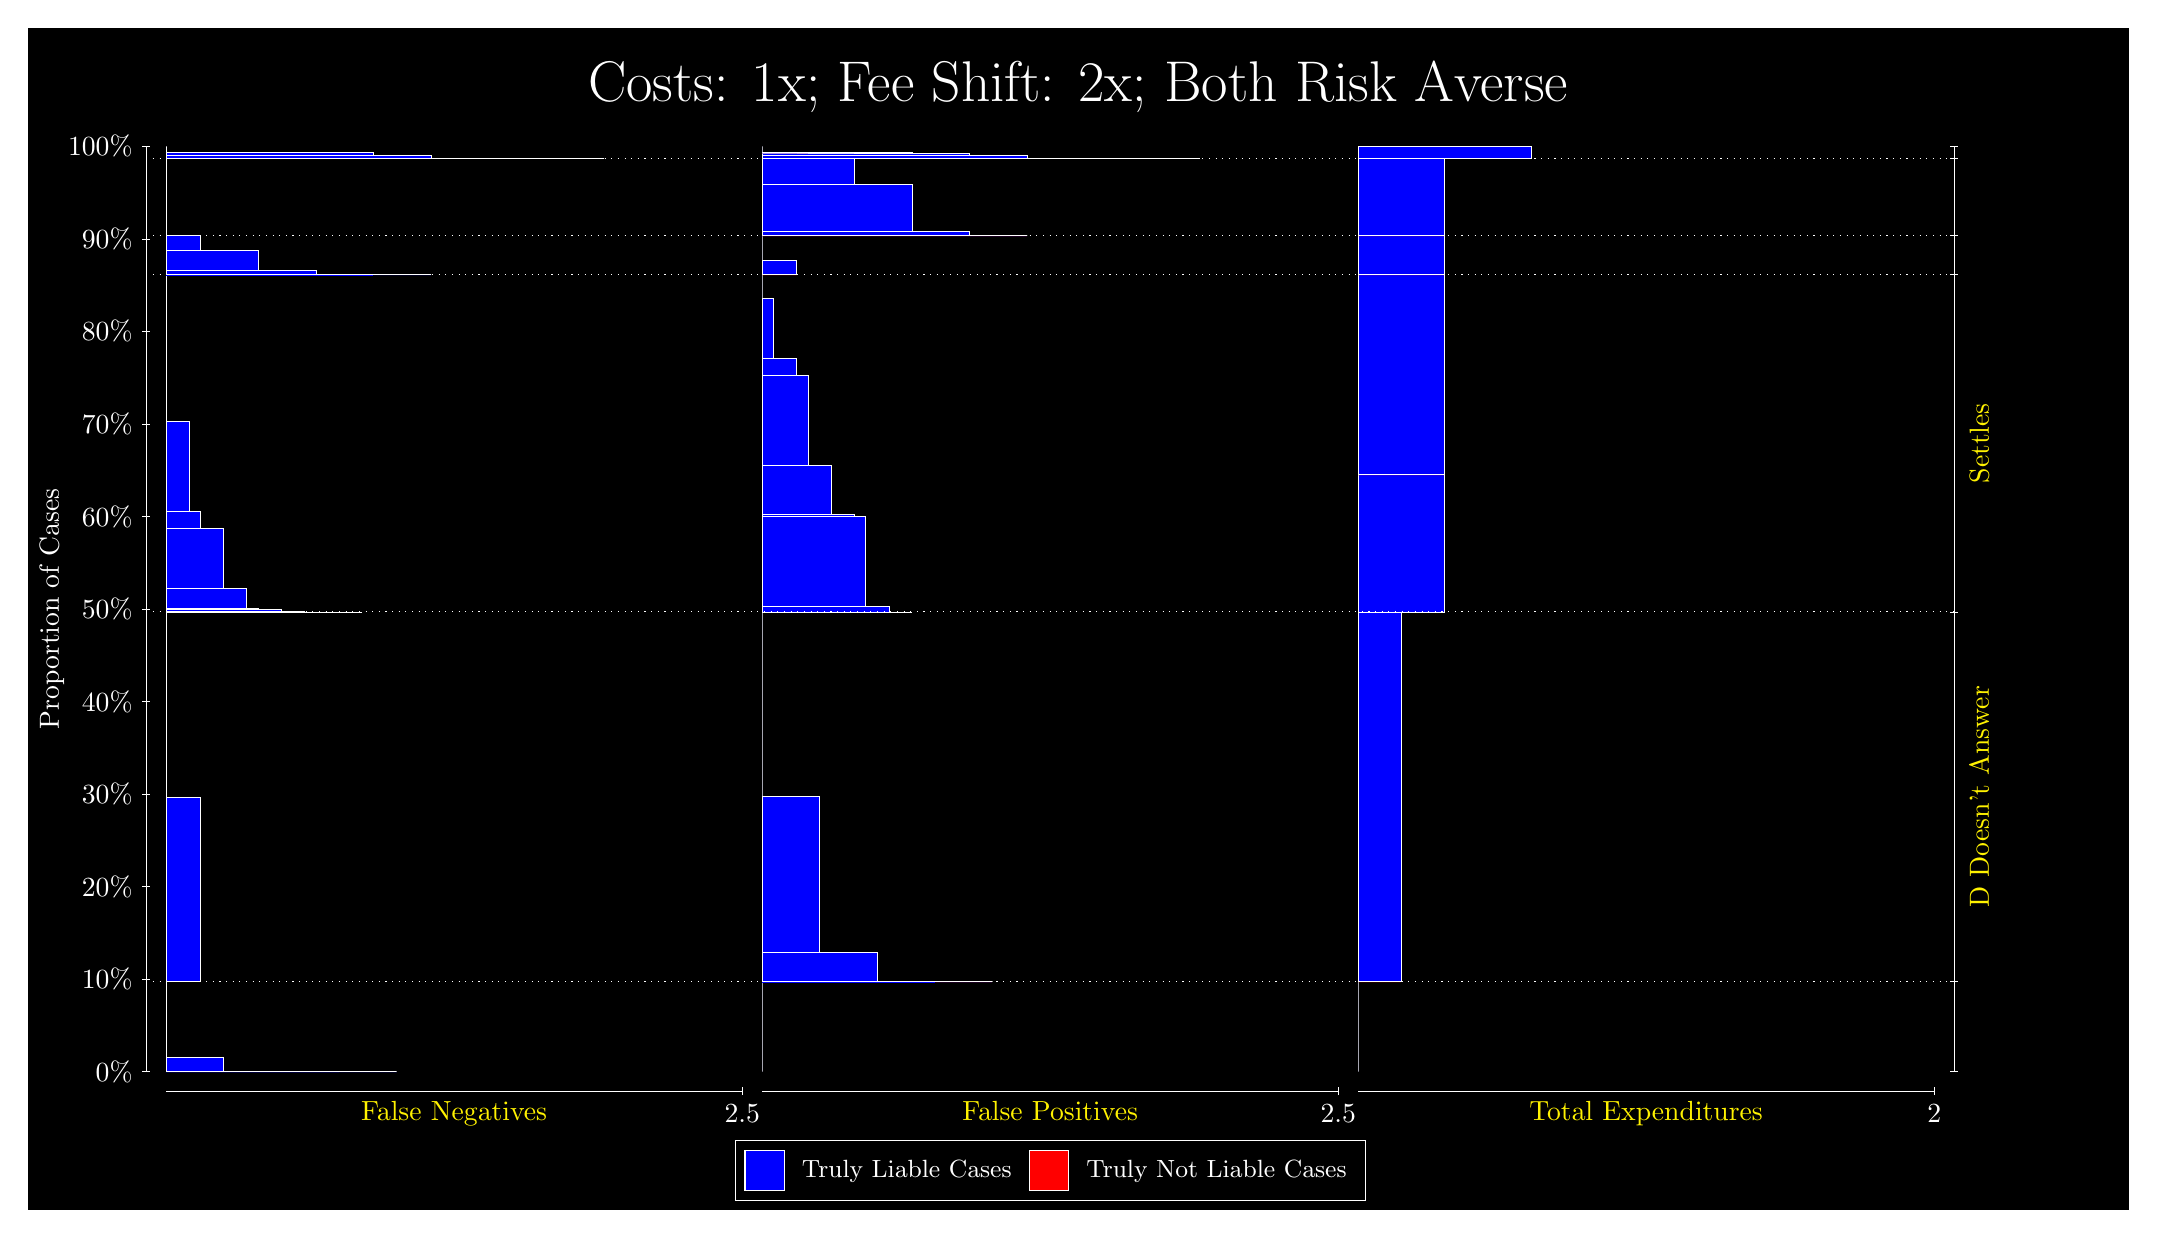
\begin{tikzpicture}
\draw[fill=black] (0,0) rectangle (26.667,15);
\draw[text=white] (0,13.5) rectangle (26.667,15) node[midway] {\huge Costs: 1x; Fee Shift: 2x; Both Risk Averse};
\draw[white, very thin] (1.5,1.75) -- (1.5,13.5);
\node[rotate=90, text=white, anchor=center] at (0.3, 7.625) {Proportion of Cases};
\draw[white, very thin] (1.45,1.75) -- (1.55,1.75);
\node[text=white, anchor=east] at (1.45, 1.75) {0\%};
\draw[white, very thin] (1.45,2.925) -- (1.55,2.925);
\node[text=white, anchor=east] at (1.45, 2.925) {10\%};
\draw[white, very thin] (1.45,4.1) -- (1.55,4.1);
\node[text=white, anchor=east] at (1.45, 4.1) {20\%};
\draw[white, very thin] (1.45,5.275) -- (1.55,5.275);
\node[text=white, anchor=east] at (1.45, 5.275) {30\%};
\draw[white, very thin] (1.45,6.45) -- (1.55,6.45);
\node[text=white, anchor=east] at (1.45, 6.45) {40\%};
\draw[white, very thin] (1.45,7.625) -- (1.55,7.625);
\node[text=white, anchor=east] at (1.45, 7.625) {50\%};
\draw[white, very thin] (1.45,8.8) -- (1.55,8.8);
\node[text=white, anchor=east] at (1.45, 8.8) {60\%};
\draw[white, very thin] (1.45,9.975) -- (1.55,9.975);
\node[text=white, anchor=east] at (1.45, 9.975) {70\%};
\draw[white, very thin] (1.45,11.15) -- (1.55,11.15);
\node[text=white, anchor=east] at (1.45, 11.15) {80\%};
\draw[white, very thin] (1.45,12.325) -- (1.55,12.325);
\node[text=white, anchor=east] at (1.45, 12.325) {90\%};
\draw[white, very thin] (1.45,13.5) -- (1.55,13.5);
\node[text=white, anchor=east] at (1.45, 13.5) {100\%};

\draw[white, very thin] (24.457,1.75) -- (24.457,13.5);
\draw[white, very thin] (24.407,1.75) -- (24.507,1.75);
\node[anchor=west] at (24.407, 1.75) {};
\draw[white, very thin] (24.407,2.8901) -- (24.507,2.8901);
\node[anchor=west] at (24.407, 2.8901) {};
\draw[white, very thin] (24.407,7.5885) -- (24.507,7.5885);
\node[anchor=west] at (24.407, 7.5885) {};
\draw[white, very thin] (24.407,11.87) -- (24.507,11.87);
\node[anchor=west] at (24.407, 11.87) {};
\draw[white, very thin] (24.407,12.365) -- (24.507,12.365);
\node[anchor=west] at (24.407, 12.365) {};
\draw[white, very thin] (24.407,13.346) -- (24.507,13.346);
\node[anchor=west] at (24.407, 13.346) {};
\draw[white, very thin] (24.407,13.5) -- (24.507,13.5);
\node[anchor=west] at (24.407, 13.5) {};

\draw[white, very thin, fill=blue] (1.75,1.75) rectangle (4.6775,1.75);
\draw[white, very thin, fill=blue] (1.75,1.75) rectangle (3.9457,1.75);
\draw[white, very thin, fill=blue] (1.75,1.75) rectangle (3.2138,1.7516);
\draw[white, very thin, fill=blue] (1.75,1.7516) rectangle (2.4819,1.9367);
\draw[white, very thin, fill=red] (1.75,1.9367) rectangle (1.75,1.9367);
\draw[white, very thin, fill=blue] (1.75,1.9367) rectangle (1.75,2.8901);
\draw[white, very thin, fill=blue] (1.75,2.8901) rectangle (2.1891,5.2363);
\draw[white, very thin, fill=red] (1.75,5.2363) rectangle (1.75,5.2363);
\draw[white, very thin, fill=blue] (1.75,5.2363) rectangle (1.75,7.5885);
\draw[white, very thin, fill=blue] (1.75,7.5885) rectangle (4.2384,7.5885);
\draw[white, very thin, fill=blue] (1.75,7.5885) rectangle (3.9457,7.5885);
\draw[white, very thin, fill=blue] (1.75,7.5885) rectangle (3.6529,7.5885);
\draw[white, very thin, fill=blue] (1.75,7.5885) rectangle (3.5065,7.5933);
\draw[white, very thin, fill=blue] (1.75,7.5933) rectangle (3.2138,7.6206);
\draw[white, very thin, fill=blue] (1.75,7.6206) rectangle (2.921,7.6314);
\draw[white, very thin, fill=blue] (1.75,7.6314) rectangle (2.7746,7.8852);
\draw[white, very thin, fill=blue] (1.75,7.8852) rectangle (2.4819,8.6552);
\draw[white, very thin, fill=blue] (1.75,8.6552) rectangle (2.1891,8.8713);
\draw[white, very thin, fill=blue] (1.75,8.8713) rectangle (2.0428,10.012);
\draw[white, very thin, fill=red] (1.75,10.012) rectangle (1.75,10.012);
\draw[white, very thin, fill=blue] (1.75,10.012) rectangle (1.75,11.87);
\draw[white, very thin, fill=blue] (1.75,11.87) rectangle (5.1167,11.87);
\draw[white, very thin, fill=blue] (1.75,11.87) rectangle (4.3848,11.871);
\draw[white, very thin, fill=blue] (1.75,11.871) rectangle (3.6529,11.924);
\draw[white, very thin, fill=blue] (1.75,11.924) rectangle (2.921,12.18);
\draw[white, very thin, fill=blue] (1.75,12.18) rectangle (2.1891,12.365);
\draw[white, very thin, fill=red] (1.75,12.365) rectangle (1.75,12.365);
\draw[white, very thin, fill=blue] (1.75,12.365) rectangle (2.1891,12.369);
\draw[white, very thin, fill=red] (1.75,12.369) rectangle (1.75,12.369);
\draw[white, very thin, fill=blue] (1.75,12.369) rectangle (1.75,13.346);
\draw[white, very thin, fill=blue] (1.75,13.346) rectangle (7.3123,13.346);
\draw[white, very thin, fill=blue] (1.75,13.346) rectangle (6.5805,13.346);
\draw[white, very thin, fill=blue] (1.75,13.346) rectangle (5.8486,13.348);
\draw[white, very thin, fill=blue] (1.75,13.348) rectangle (5.1167,13.38);
\draw[white, very thin, fill=blue] (1.75,13.38) rectangle (4.3848,13.422);
\draw[white, very thin, fill=blue] (1.75,13.422) rectangle (3.6529,13.426);
\draw[white, very thin, fill=blue] (1.75,13.426) rectangle (3.0674,13.426);
\draw[white, very thin, fill=blue] (1.75,13.426) rectangle (2.921,13.426);
\draw[white, very thin, fill=blue] (1.75,13.426) rectangle (2.3355,13.426);
\draw[white, very thin, fill=red] (1.75,13.426) rectangle (1.75,13.426);
\draw[white, very thin, fill=blue] (1.75,13.426) rectangle (1.75,13.5);
\draw[white, very thin, fill=red] (9.3189,1.75) rectangle (9.3189,1.75);
\draw[white, very thin, fill=blue] (9.3189,1.75) rectangle (9.3189,2.8901);
\draw[white, very thin, fill=red] (9.3189,2.8901) rectangle (12.246,2.8901);
\draw[white, very thin, fill=blue] (9.3189,2.8901) rectangle (12.246,2.8901);
\draw[white, very thin, fill=blue] (9.3189,2.8901) rectangle (11.515,2.893);
\draw[white, very thin, fill=blue] (9.3189,2.893) rectangle (10.783,3.2656);
\draw[white, very thin, fill=blue] (9.3189,3.2656) rectangle (10.051,5.2423);
\draw[white, very thin, fill=blue] (9.3189,5.2423) rectangle (9.3189,7.5885);
\draw[white, very thin, fill=red] (9.3189,7.5885) rectangle (11.222,7.5885);
\draw[white, very thin, fill=blue] (9.3189,7.5885) rectangle (11.222,7.5885);
\draw[white, very thin, fill=red] (9.3189,7.5885) rectangle (10.929,7.5885);
\draw[white, very thin, fill=blue] (9.3189,7.5885) rectangle (10.929,7.6586);
\draw[white, very thin, fill=red] (9.3189,7.6586) rectangle (10.636,7.6586);
\draw[white, very thin, fill=blue] (9.3189,7.6586) rectangle (10.636,8.7988);
\draw[white, very thin, fill=blue] (9.3189,8.7988) rectangle (10.49,8.8238);
\draw[white, very thin, fill=blue] (9.3189,8.8238) rectangle (10.197,9.4463);
\draw[white, very thin, fill=blue] (9.3189,9.4463) rectangle (9.9044,10.587);
\draw[white, very thin, fill=blue] (9.3189,10.587) rectangle (9.758,10.803);
\draw[white, very thin, fill=blue] (9.3189,10.803) rectangle (9.4652,11.573);
\draw[white, very thin, fill=blue] (9.3189,11.573) rectangle (9.3189,11.87);
\draw[white, very thin, fill=red] (9.3189,11.87) rectangle (9.758,11.87);
\draw[white, very thin, fill=blue] (9.3189,11.87) rectangle (9.758,12.055);
\draw[white, very thin, fill=blue] (9.3189,12.055) rectangle (9.3189,12.365);
\draw[white, very thin, fill=red] (9.3189,12.365) rectangle (12.686,12.365);
\draw[white, very thin, fill=blue] (9.3189,12.365) rectangle (12.686,12.365);
\draw[white, very thin, fill=blue] (9.3189,12.365) rectangle (11.954,12.416);
\draw[white, very thin, fill=blue] (9.3189,12.416) rectangle (11.222,13.014);
\draw[white, very thin, fill=blue] (9.3189,13.014) rectangle (10.49,13.342);
\draw[white, very thin, fill=blue] (9.3189,13.342) rectangle (9.758,13.346);
\draw[white, very thin, fill=red] (9.3189,13.346) rectangle (14.881,13.346);
\draw[white, very thin, fill=blue] (9.3189,13.346) rectangle (14.881,13.346);
\draw[white, very thin, fill=red] (9.3189,13.346) rectangle (14.149,13.346);
\draw[white, very thin, fill=blue] (9.3189,13.346) rectangle (14.149,13.346);
\draw[white, very thin, fill=red] (9.3189,13.346) rectangle (13.417,13.346);
\draw[white, very thin, fill=blue] (9.3189,13.346) rectangle (13.417,13.349);
\draw[white, very thin, fill=red] (9.3189,13.349) rectangle (12.686,13.349);
\draw[white, very thin, fill=blue] (9.3189,13.349) rectangle (12.686,13.381);
\draw[white, very thin, fill=blue] (9.3189,13.381) rectangle (11.954,13.417);
\draw[white, very thin, fill=blue] (9.3189,13.417) rectangle (11.222,13.42);
\draw[white, very thin, fill=blue] (9.3189,13.42) rectangle (10.49,13.42);
\draw[white, very thin, fill=red] (9.3189,13.42) rectangle (9.9044,13.42);
\draw[white, very thin, fill=blue] (9.3189,13.42) rectangle (9.9044,13.42);
\draw[white, very thin, fill=blue] (9.3189,13.42) rectangle (9.758,13.42);
\draw[white, very thin, fill=red] (9.3189,13.42) rectangle (9.3189,13.42);
\draw[white, very thin, fill=blue] (9.3189,13.42) rectangle (9.3189,13.5);
\draw[white, very thin, fill=red] (16.888,1.75) rectangle (16.888,1.75);
\draw[white, very thin, fill=blue] (16.888,1.75) rectangle (16.888,2.8901);
\draw[white, very thin, fill=red] (16.888,2.8901) rectangle (17.437,2.8901);
\draw[white, very thin, fill=blue] (16.888,2.8901) rectangle (17.437,7.5885);
\draw[white, very thin, fill=red] (16.888,7.5885) rectangle (17.986,7.5885);
\draw[white, very thin, fill=blue] (16.888,7.5885) rectangle (17.986,9.3303);
\draw[white, very thin, fill=red] (16.888,9.3303) rectangle (17.986,9.3303);
\draw[white, very thin, fill=blue] (16.888,9.3303) rectangle (17.986,11.87);
\draw[white, very thin, fill=red] (16.888,11.87) rectangle (17.986,11.87);
\draw[white, very thin, fill=blue] (16.888,11.87) rectangle (17.986,12.365);
\draw[white, very thin, fill=red] (16.888,12.365) rectangle (17.986,12.365);
\draw[white, very thin, fill=blue] (16.888,12.365) rectangle (17.986,13.346);
\draw[white, very thin, fill=red] (16.888,13.346) rectangle (19.083,13.346);
\draw[white, very thin, fill=blue] (16.888,13.346) rectangle (19.083,13.5);
\draw[white, dotted] (1.5,2.8901) -- (24.457,2.8901);
\draw[white, dotted] (1.5,7.5885) -- (24.457,7.5885);
\draw[white, dotted] (1.5,11.87) -- (24.457,11.87);
\draw[white, dotted] (1.5,12.365) -- (24.457,12.365);
\draw[white, dotted] (1.5,13.346) -- (24.457,13.346);
\draw[white, very thin] (1.75,1.5) -- (9.0689,1.5);
\node[text=yellow, anchor=north] at (5.4094, 1.5) {False Negatives};
\draw[white, very thin] (9.0689,1.45) -- (9.0689,1.55);
\node[text=white, anchor=north] at (9.0689, 1.45) {2.5};

\draw[white, very thin] (9.3189,1.5) -- (16.638,1.5);
\node[text=yellow, anchor=north] at (12.978, 1.5) {False Positives};
\draw[white, very thin] (16.638,1.45) -- (16.638,1.55);
\node[text=white, anchor=north] at (16.638, 1.45) {2.5};

\draw[white, very thin] (16.888,1.5) -- (24.207,1.5);
\node[text=yellow, anchor=north] at (20.547, 1.5) {Total Expenditures};
\draw[white, very thin] (24.207,1.45) -- (24.207,1.55);
\node[text=white, anchor=north] at (24.207, 1.45) {2};


\node[text=yellow, centered, rotate=90] at (24.777, 5.2393) {D Doesn't Answer};
\node[text=yellow, centered, rotate=90] at (24.777, 9.729) {Settles};




\draw (12.978300999999998,1.5) node[draw=none] (baseCoordinate) {};
\begin{scope}[align=center]
        \matrix[scale=0.5, draw=white, below=0.5cm of baseCoordinate, nodes={draw}, column sep=0.1cm]{
            \node[rectangle, draw, minimum width=0.5cm, minimum height=0.5cm, fill=blue] {}; &
            \node[draw=none, font=\small, text=white] (B) {Truly Liable Cases}; &
            \node[rectangle, draw, minimum width=0.5cm, minimum height=0.5cm, fill=red] {}; &
            \node[draw=none, font=\small, text=white] (B) {Truly Not Liable Cases}; \\
            };
\end{scope}

\end{tikzpicture}
\end{document}